\clearpage
\setcounter{page}{1}
\maketitlesupplementary

\section{Synthetic Dataset Parameters}
\label{sec:dataset_params}

\cref{tab:in_dist_sampling,tab:holoocean_standard_sampling,tab:holoocean_rough_sampling} summarize the empirical sampling ranges observed in each dataset. We report the minimum and maximum values across the full split for each setting. Note that the amplitude refers to the peak-to-trough height (maximum minus minimum elevation). Although we targeted matching configuration ranges between the synthetic and HoloOcean standard datasets, integration with HoloOcean resulted in slightly different realized parameter bounds. We present samples from each dataset in Fig.~\ref{fig:dset_samples}.

\begin{table}[t]
  \centering
  \caption{\centering
    { In-distribution synthetic sampling parameters.}\\
    Empirical min/max over 10{,}000 train, 200 val, \\ and 200 test samples.}
  \label{tab:in_dist_sampling}
  \begin{tabular}{@{}lcc@{}}
    \toprule
    Parameter & Min & Max \\
    \midrule
    \multicolumn{3}{@{}l}{\textbf{Sensor parameters}} \\
    Azimuth spread (\(^\circ\))      & 10.0 & 19.0 \\
    Start range (m)                  & 1.53 & 4.97 \\
    End range (m)                    & 3.80 & 7.50 \\
    Range coverage (m)               & 2.03 & 5.49 \\
    Range bins                       & 380  & 512  \\
    Azimuth bins                     & 36   & 64   \\
    Elevation spread (\(^\circ\))    & 10.0 & 19.0 \\
    \midrule
    \multicolumn{3}{@{}l}{\textbf{Seafloor parameters}} \\
    Amplitude (cm)                   & 2.01 & 9.98 \\
    Frequency (\(\text{m}^{-1}\))   & 2.00 & 15.0 \\
    Ground tilt (\(^\circ\))         & 6.87 & 38.0 \\
    \bottomrule
  \end{tabular}
\end{table}

\begin{table}[t]
  \centering
  \caption{\centering
    { HoloOcean standard sampling parameters.}\\
    Empirical min/max over 149 samples.}
  \label{tab:holoocean_standard_sampling}
  \begin{tabular}{@{}lcc@{}}
    \toprule
    Parameter & Min & Max \\
    \midrule
    \multicolumn{3}{@{}l}{\textbf{Sensor parameters}} \\
    Azimuth spread (\(^\circ\))      & 10.0 & 29.0 \\
    Start range (m)                  & 1.01 & 5.99 \\
    End range (m)                    & 4.16 & 8.50 \\
    Range coverage (m)               & 2.51 & 5.50 \\
    Range bins                       & 512  & 512  \\
    Azimuth bins                     & 48   & 48   \\
    Elevation spread (\(^\circ\))    & 10.0 & 29.0 \\
    \midrule
    \multicolumn{3}{@{}l}{\textbf{Seafloor parameters}} \\
    Amplitude (cm)                   & 1.03 & 7.97 \\
    Frequency (\(\text{m}^{-1}\))   & 1.00 & 4.00 \\
    Ground tilt (\(^\circ\))         & 6.59 & 47.23 \\
    \bottomrule
  \end{tabular}
\end{table}

\begin{table}[t]
  \centering
  \caption{\centering
    { HoloOcean rough-terrain sampling parameters.}\\
    Empirical min/max over 35 samples.}
  \label{tab:holoocean_rough_sampling}
  \begin{tabular}{@{}lcc@{}}
    \toprule
    Parameter & Min & Max \\
    \midrule
    \multicolumn{3}{@{}l}{\textbf{Sensor parameters}} \\
    Azimuth spread (\(^\circ\))      & 10.0 & 29.0 \\
    Start range (m)                  & 5.14 & 7.98 \\
    End range (m)                    & 8.56 & 12.62 \\
    Range coverage (m)               & 3.12 & 4.97 \\
    Range bins                       & 512  & 512  \\
    Azimuth bins                     & 48   & 48   \\
    Elevation spread (\(^\circ\))    & 11.0 & 28.0 \\
    \midrule
    \multicolumn{3}{@{}l}{\textbf{Seafloor parameters}} \\
    Amplitude (cm)                   & 10.0 & 15.9 \\
    Frequency (\(\text{m}^{-1}\))   & 1.00 & 3.50 \\
    Ground tilt (\(^\circ\))         & 14.4 & 51.1 \\
    \bottomrule
  \end{tabular}
\end{table}

We refer to the synthetic dataset generated with our own forward model as ``in-distribution,'' since the CNN is trained and evaluated on samples drawn from the same simulator and parameter ranges. The HoloOcean datasets differ in simulator, sensor model, and realized parameter ranges, and are therefore treated as out of distribution, even though the underlying seafloor prior (Perlin height fields) is shared.


\section{Hyperparameters and Configs}
\label{sec:hyperparameters}

\begin{table*}[t]
    \centering
    \caption{\centering
        Key hyperparameters for differentiable rendering and inverse reconstruction.}
    \label{tab:hyperparams}
    \begin{tabular}{@{}lll@{}}
        \toprule
        Component & Parameter & Default / range \\
        \midrule
        Forward model / renderer
        & Elevation samples \(n_\mathrm{el}\) &
            \(6\,n_\mathrm{bins}\) per azimuth beam \\
        & Gaussian bin spread \(\sigma_\mathrm{bins}\) &
            \num{0.5} - \num{1.0} bins \\
        & Near-range padding &
            4 bins in front of \(r_\mathrm{min}\) \\
        & Two-way geometric spreading &
            \(1/r^4\) correction (TVG undo optional) \\
        & TVG exponent &
            \num{3.2} - \num{4.0} \\
        % & Additional attenuation coefficient &
            % \num{0} - \num{1e-2} (toggleable) \\
        & Diffuse exponent \(\gamma\) &
            \num{1.0} - \num{2.0} \\
        & Specular spread \(\sigma_\mathrm{spec}\) &
            \(5^\circ - 10^\circ\) \\
        \midrule
        Seafloor / intersections
        & Collision sharpness \(\alpha\) &
            \num{2500} - \num{4500} \\
        & HT plane coverage &
            \(90\%\) of elevation span \\
        & GV sampling range &
            60–97.5\% of elevation span \\
        \midrule
        Image processing
        & Azimuth gains &
            One scalar per beam \\
        & Gain learning rate &
            \(0 \rightarrow 10^{-1}\) (after warmup) \\
        \midrule
        Optimization
        & Steps per frame &
            \num{100}-\num{300} \\
        & TV weight \(\lambda_\mathrm{TV}\) &
            \num{0.0} - \num{1.0} \\
        & Optimizer &
            AdamW \\
        & Geometry learning rate &
            \(10^{-4}\) \\
        & Warmup steps \(n_\mathrm{warmup}\) &
            \num{30} (freeze gains) \\
        \bottomrule
    \end{tabular}
\end{table*}

Table~\ref{tab:hyperparams} provides the key hyperparameter ranges for our differentiable renderer and inverse reconstructions. We choose the elevation sampling density, \(n_\text{el}\), so that each beam approximates a continuous vertical fan. The near-range padding adds out-of-view bins to the front of the height field to prevent artifacts from offscreen occlusions. The ranges listed here include values that we found stable in practice. We did not tune these heavily for each dataset.


\section{Additional Ablations}
\label{sec:more_ablations}
To further identify the optimal configurations of our system, and the benefits of the generic viewpoint approach, we perform additional ablations over the learning rate, optimization steps, and generic viewpoint coverage.

\subsection{Learning Rate Ablation}
\label{sec:lr_ablate}

To study the tradeoff between optimization budget and reconstruction accuracy we sweep the geometry learning rate across several orders of magnitude and vary the number of gradient steps. For each combination we fit the polar height field on the HoloOcean rough terrain dataset using the generic viewpoint (GV) approach and a fixed TV weight of \num{0.1}. We report the 3D MSE over the test set.

\begin{table*}[h]
  \centering
  \captionsetup{width=0.85\linewidth}
  \caption{\centering
    HoloOcean Rough Terrain 3D MSE (cm$^2$, ↓) scores across optimization steps and learning rates.
    Evaluated using the generic viewpoint (GV) approach with \(\lambda_\text{TV}=0.1\).
    For each number of steps, the best learning rate is shown in bold. The overall optimal performance is achieved at 200 steps with a learning rate of \num{1e-4}.
  }
  \label{tab:steps_lr_ablation_mse}
  \begin{tabular}{@{}lccccc@{}}
    \toprule
    Steps / LR &
    $1\times10^{-6}$ &
    $1\times10^{-5}$ &
    $5\times10^{-5}$ &
    $1\times10^{-4}$ &
    $5\times10^{-4}$ \\
    % $1\times10^{-3}$ \\
    \midrule
    50  & 7.034 & 6.423 & 5.169 & \textbf{4.834} & 5.984 \\ %& 21.686 \\
    75  & 6.998 & 6.147 & 4.808 & \textbf{4.529} & 6.160 \\ %& 26.547 \\
    100 & 6.960 & 5.916 & 4.595 & \textbf{4.364} & 6.750 \\ %& 31.843 \\
    150 & 6.886 & 5.556 & 4.370 & \textbf{4.219} & 9.056 \\ %& 42.364 \\
    200 & 6.813 & 5.292 & 4.279 & \textit{\textbf{4.200}} & 12.398 \\ %& 52.188 \\
    300 & 6.673 & 4.938 & \textbf{4.286} & 4.325 & 21.012 \\ %& 69.325 \\
    400 & 6.540 & 4.721 & \textbf{4.399} & 4.568 & 30.553 \\ %& 84.699 \\
    \bottomrule
  \end{tabular}
\end{table*}

As shown in Tab.~\ref{tab:steps_lr_ablation_mse}, very small learning rates converge slowly and leave significant error even after many steps, while very large learning rates overshoot and degrade performance. The optimization remains stable up to a learning rate around \(5\times10^{-4}\), where it begins to create extreme geometry resulting in large error. A mid–range value around \(10^{-4}\) provides a stable compromise. It typically achieves optimal accuracy around \num{150}-\num{200} steps.

\subsection{Generic Viewpoint}
\label{sec:gv_ablate}

The generic–viewpoint prior is implemented by sampling base–plane orientations that cover a specified fraction of the sonar elevation span. At each optimization step, we sample a random plane within the specified range (from min. coverage to full coverage) and apply the corresponding tilt to the latent seafloor. This encourages reconstructions that remain consistent under small changes to the supporting plane.

To test how this prior performs under different sampling ranges, we vary the minimum coverage of the elevation span and evaluate the 3D MSE on all three datasets. Low coverage allows shallow planes that only intersect part of the range. High coverage forces the plane to span most of the elevation arc, which  restricts the feasible orientations.

\begin{table*}[h]
  \centering
  \caption{\centering
    {3D MSE (cm$^2$, ↓) across different generic viewpoint sampling schemes.}
    Evaluated with \(\lambda_\text{TV}=0.1\).
  }
  \label{tab:gv_ablate}
  \begin{tabular}{@{}lccc@{}}
    \toprule
    GV Min. Coverage &
    In-Distribution &
    HoloOcean &
    HO Rough \\
    \midrule
    0\%  & 0.821 & 1.036 & 4.958 \\
    10\% & 0.792 & 0.963 & 4.633 \\
    20\% & 0.683 & 0.908 & 4.325 \\
    30\% & 0.632 & 0.890 & 4.223 \\
    40\% & 0.601 & \textbf{0.885} & \textbf{4.165} \\
    50\% & 0.583 & 0.894 & 4.174 \\
    60\% & 0.578 & 0.907 & 4.213 \\
    70\% & \textbf{0.577} & 0.917 & 4.285 \\
    80\% & 0.581 & 0.933 & 4.384 \\
    90\% & 0.599 & 0.960 & 4.532 \\
    \bottomrule
  \end{tabular}
\end{table*}

As shown in Tab.~\ref{tab:gv_ablate}, the generic viewpoint prior remains stable across all sampling schemes. However, it clearly benefits from limiting very shallow planes, likely due to the sparse sampling and extreme geometry which occurs in this zone. Additionally, near very high coverage restrictions (around 90\%) the model performs similarly to the high-tilt approach, since we are no longer sampling over a broad range of small tilt variations. The best performance in-distribution occurs when we sample from a minimum coverage of 70\%, and for both HoloOcean datasets the best performance occurs when the minimum coverage is 40\%.

\section{Runtime and Scaling}
\label{sec:runtime_memory}

We profile the runtime and GPU memory usage of our differentiable sonar renderer and single-frame inversion on a desktop RTX~5090 GPU. We vary the number of range and azimuth bins around typical imaging sonar settings (Range $\in \{300, 400, 500, 600\}$, Azimuth $\in \{48, 96, 128\}$). For each configuration we report the average forward render time, the wall-clock time required to complete a full optimization of a single frame with 150 gradient steps, and the peak GPU memory recorded by PyTorch during the run.

We provide results at two elevation sampling levels. In the first level we cast 1500 elevation rays per azimuth beam. This configuration prioritizes speed and is sufficient for most of our experiments. In the second level we use 3000 rays per beam, which provides higher fidelity results, particularly when the number of range bins is large. Runtime and memory scale approximately linearly with the number of azimuth beams, the number of range bins, and the number of elevation rays.

At a realistic ARIS-like resolution of $96 \times 500$ bins, the 1500-ray rendering requires 83~ms per forward render, 12.5~s for a full 150-step reconstruction, and a peak of 9.7~GiB of GPU memory. With 3000 rays the same configuration requires 165~ms per render, 24.8~s for reconstruction, and 19.4~GiB of peak memory. The largest configuration with 3000 rays and $600 \times 128$ bins exceeds 32~GiB and does not fit in GPU memory.

\begin{table*}[]
  \centering
  \caption{\centering
    {Runtime and peak GPU memory for 1500 and 3000 elevation rays per azimuth beam on an RTX~5090 GPU}. We report average forward render time, total optimization time for 150 steps, and peak GPU memory.
    The configuration with 3000 elevation rays, 600 range bins, and 128 azimuth bins exceeds 30~GiB of memory and does not fit.}
  \label{tab:runtime_full}
  \begin{tabular}{@{}rccc@{\hspace{2em}}rccc@{}}
    \toprule
    \multicolumn{4}{c}{\(n_\mathrm{el}=1500\)} &
    \multicolumn{4}{c}{\(n_\mathrm{el}=3000\)} \\
    Range bins & Render (ms) & Optim. (s) & Peak VRAM (GiB) &
    Range bins & Render (ms) & Optim. (s) & Peak VRAM (GiB) \\
    \midrule
    \multicolumn{8}{@{}l}{\textbf{48 Azimuth Beams}} \\
    300 & 31  &  4.6 &  2.9 & 300 & 56  &  8.3 &  5.8 \\
    400 & 37  &  5.6 &  3.9 & 400 & 70  & 10.5 &  7.7 \\
    500 & 45  &  6.7 &  4.8 & 500 & 84  & 12.6 &  9.7 \\
    600 & 52  &  7.8 &  5.8 & 600 & 98  & 14.8 & 11.6 \\
    \midrule
    \multicolumn{8}{@{}l}{\textbf{96 Azimuth Beams}} \\
    300 & 57  &  8.6 &  5.8 & 300 & 107 & 16.1 & 11.6 \\
    400 & 71  & 10.6 &  7.7 & 400 & 134 & 20.1 & 15.5 \\
    500 & 83  & 12.5 &  9.7 & 500 & 165 & 24.8 & 19.4 \\
    600 & 100 & 15.0 & 11.6 & 600 & 197 & 29.5 & 23.2 \\
    \midrule
    \multicolumn{8}{@{}l}{\textbf{128 Azimuth Beams}} \\
    300 & 73  & 10.9 &  7.8 & 300 & 148 & 22.2 & 15.5 \\
    400 & 94  & 14.2 & 10.3 & 400 & 185 & 27.7 & 20.6 \\
    500 & 113 & 17.0 & 12.9 & 500 & 223 & 33.5 & 25.8 \\
    600 & 132 & 19.8 & 15.5 & 600 &  &   & $>$30 \\
    \bottomrule
  \end{tabular}
\end{table*}


\section{3D Reconstructions of Real Riverbeds}
\label{sec:3d_reconstructions}

In this section we present several examples of full 3D reconstructions produced by our differentiable renderer. These fits use a higher learning rate (\(3\times10^{-3}\)) and stronger TV regularization (\(\lambda_\text{TV}=0.5\)) than was used in the main paper. This choice increases contrast and occlusions in the rendered images, but also makes the underlying 3D structure easier to visualize. The full raw seafloor mesh for two real images (from Kenai Rightbank and Kenai Channel) are shown in~\cref{fig:riverA_fig1,fig:riverB_fig1} without modification. We show additional orthographic renders after applying one level of Catmull–Clark subdivision in Blender to smooth high–frequency noise in~\cref{fig:riverA_fig2,fig:riverB_fig2}.

\clearpage
\begin{figure*}[t]
    \centering
    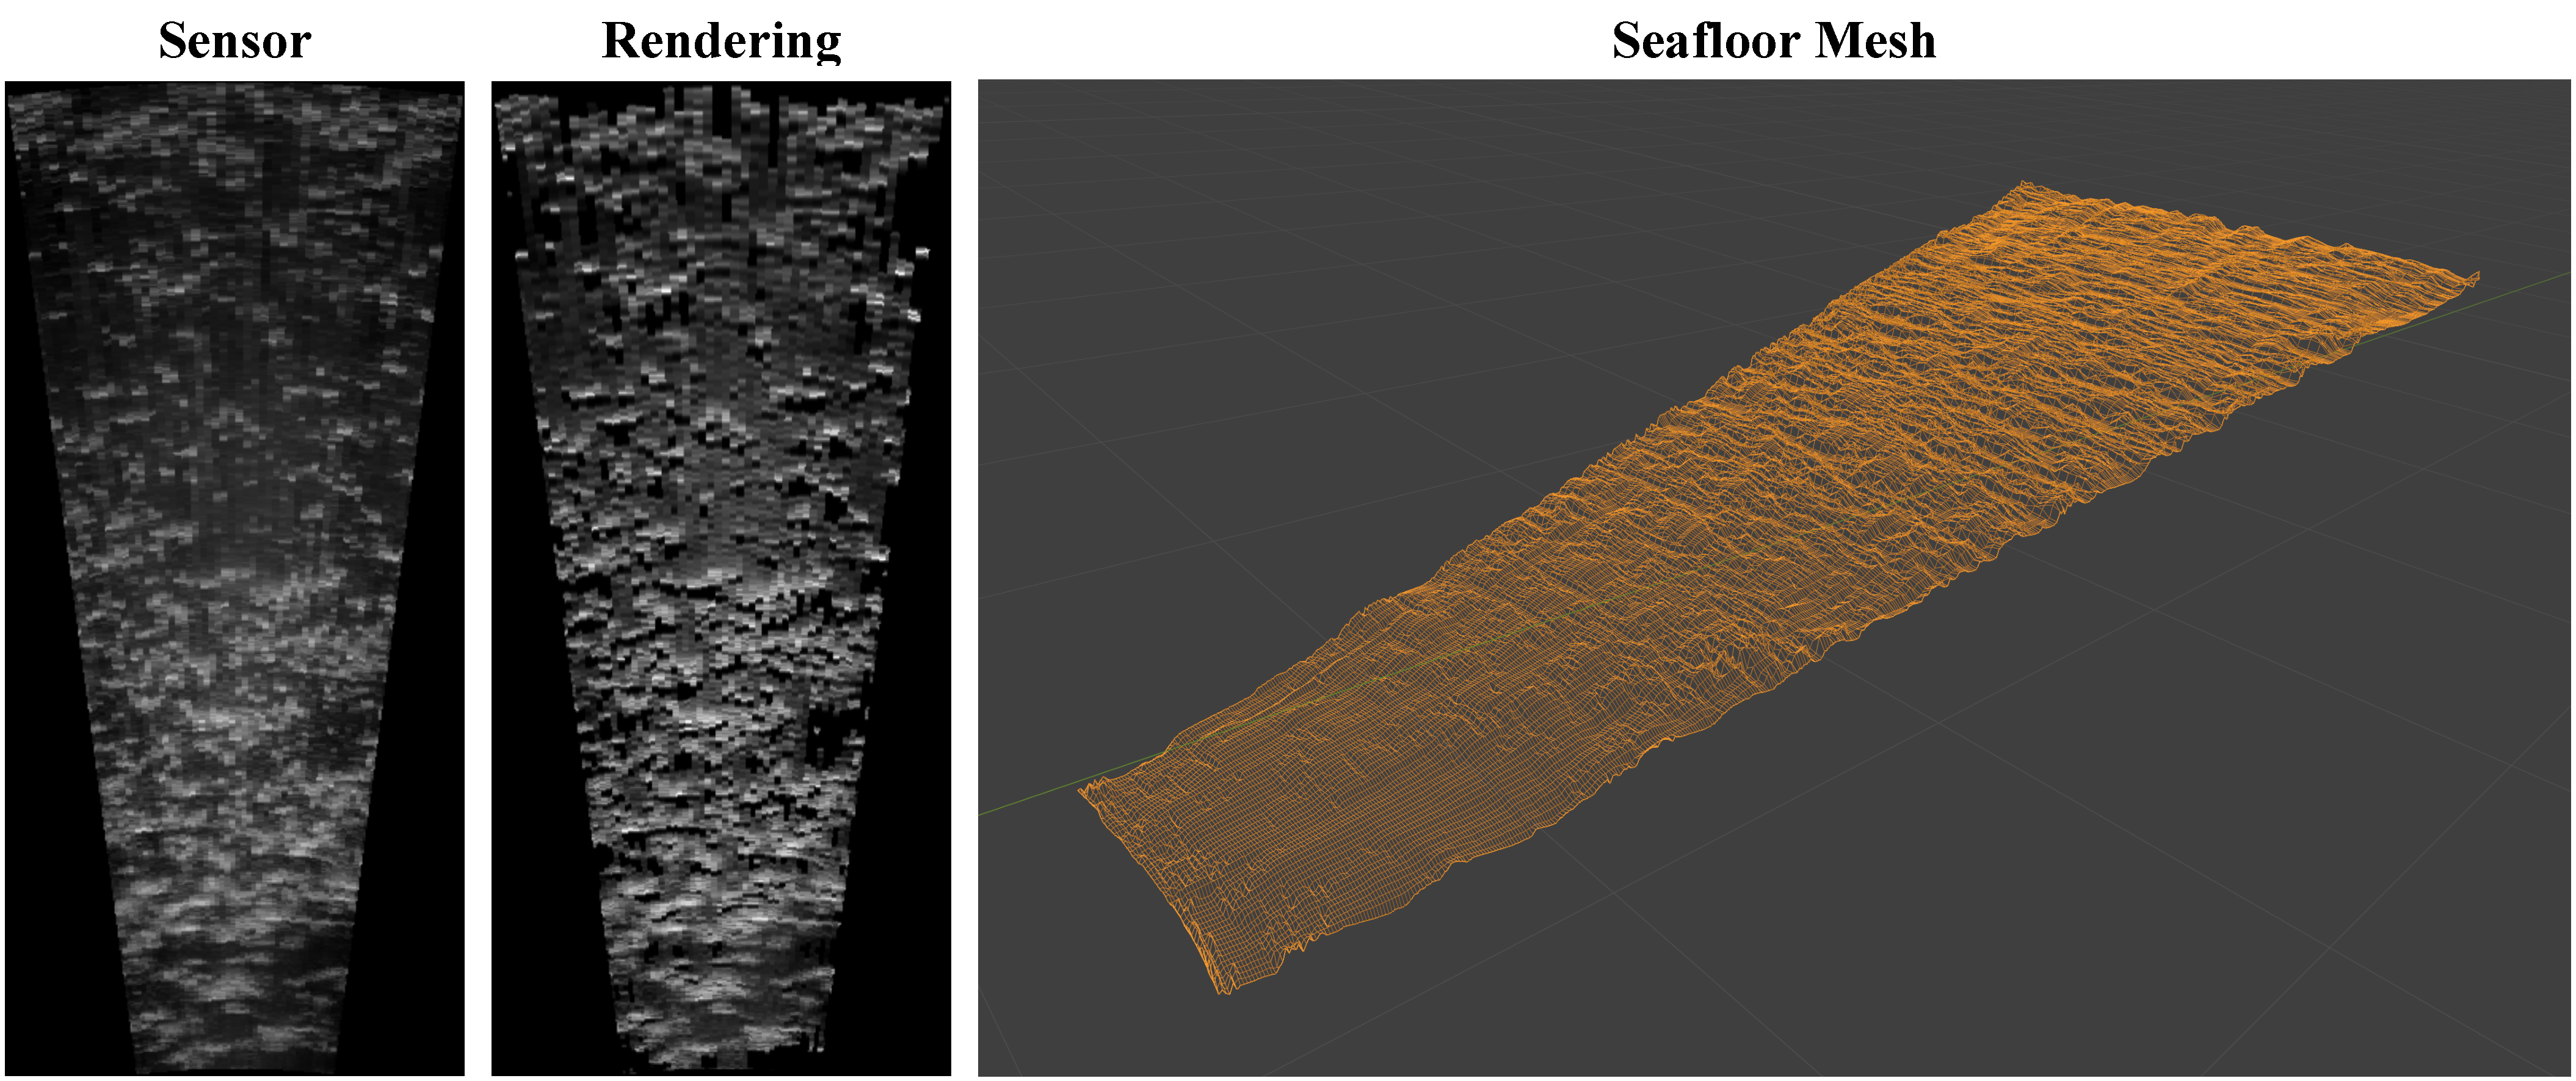
\includegraphics[width=1.0\linewidth]{figs/3d_bigview_rightbank.pdf}
    \caption{\centering {\bf Predicted seafloor mesh on Kenai Rightbank from a real sensor reading} (\textit{cf.} Sec.~\ref{sec:3d_reconstructions}).}
    \label{fig:riverA_fig1}
\end{figure*}
\begin{figure*}[t]
    \centering
    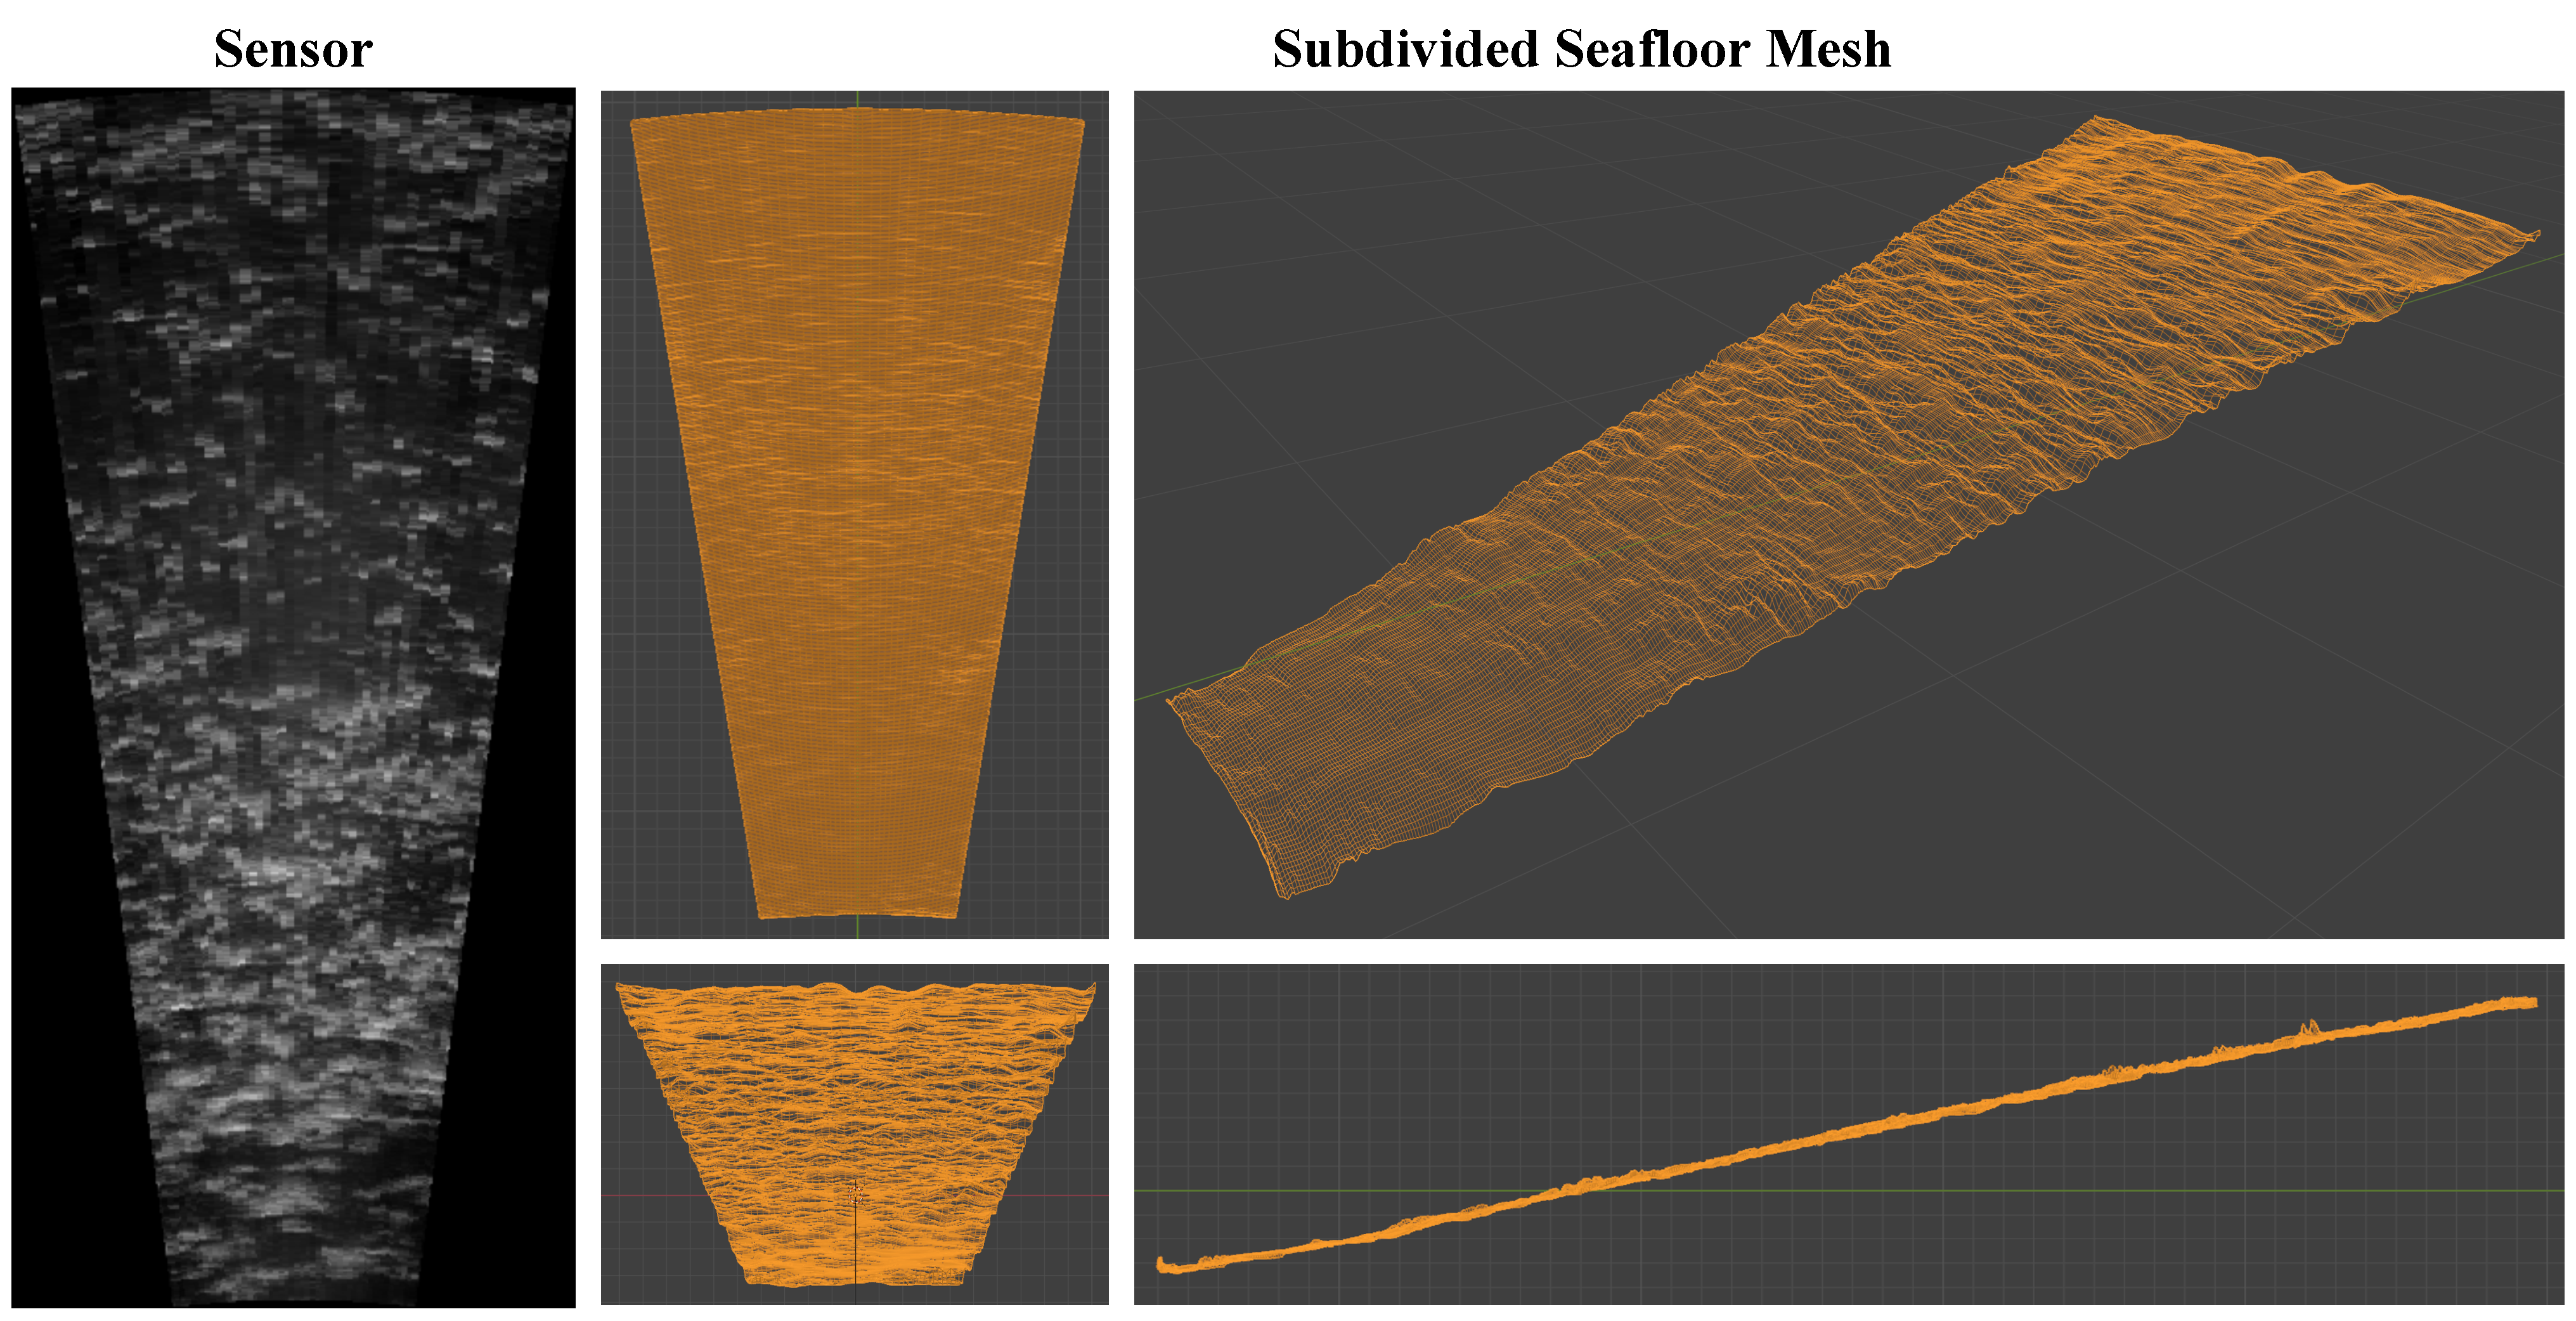
\includegraphics[width=1.0\linewidth]{figs/3d_isometrics_rb.pdf}
    \caption{\centering {\bf Additional views of the recovered seafloor geometry on Kenai Rightbank} (\textit{cf.} Sec.~\ref{sec:3d_reconstructions}). On the left we show the target again, with additional orthographic views of the recovered height field on the right after one level of Catmull–Clark subdivision in Blender (applied only for visualization).}
    \label{fig:riverA_fig2}
\end{figure*}

\begin{figure*}[t]
    \centering
    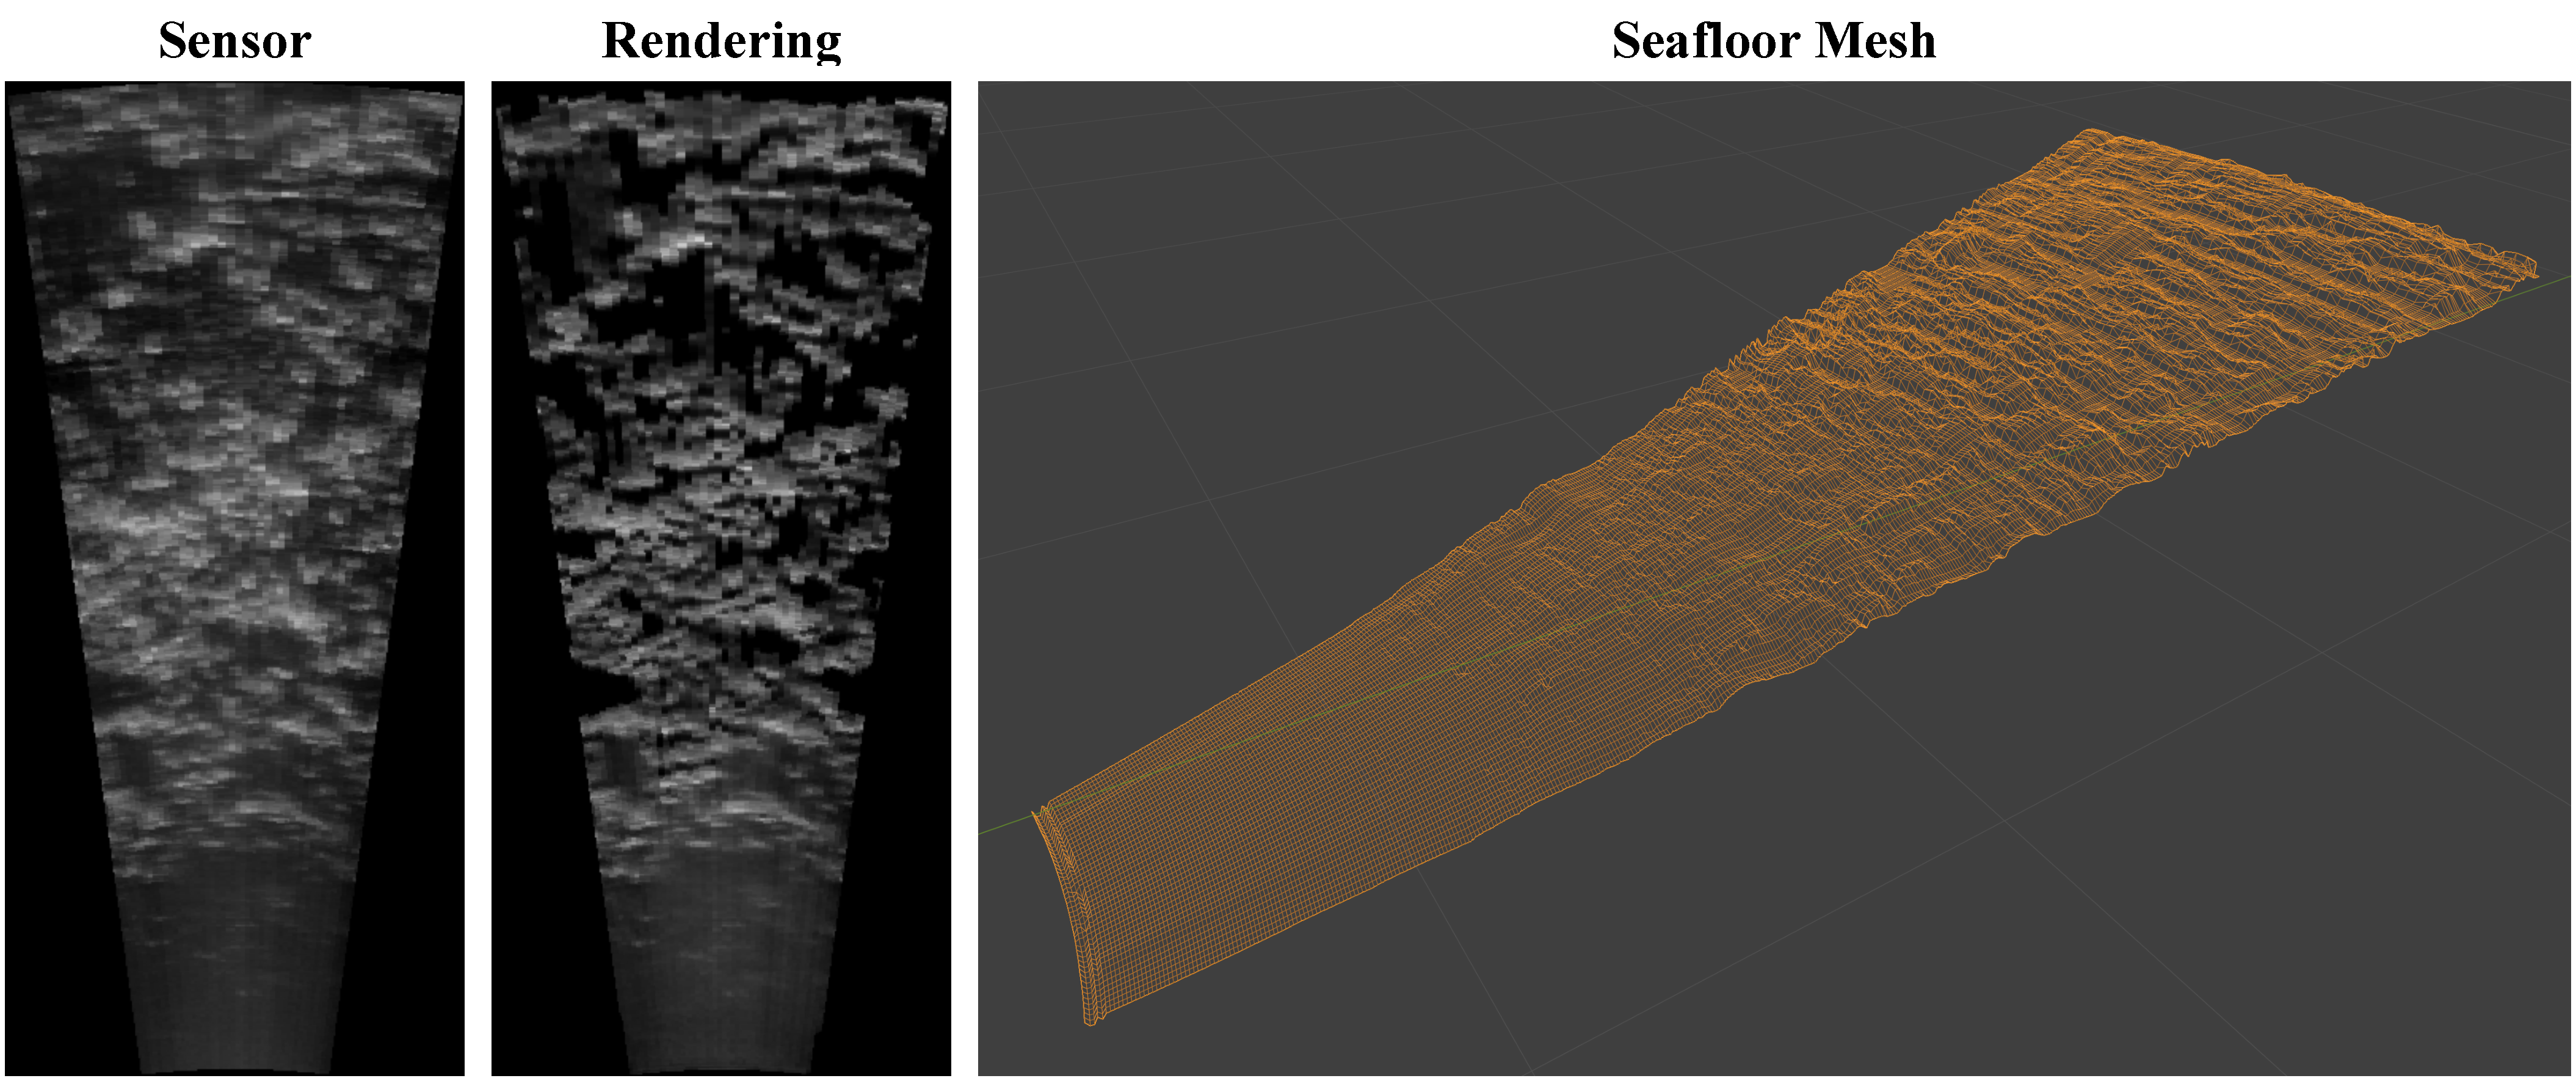
\includegraphics[width=1.0\linewidth]{figs/3d_bigview_channel.pdf}
    \caption{\centering {\bf Predicted seafloor mesh on Kenai Channel from a real sensor reading} (\textit{cf.} Sec.~\ref{sec:3d_reconstructions}).}
    \label{fig:riverB_fig1}
\end{figure*}
\begin{figure*}[t]
    \centering
    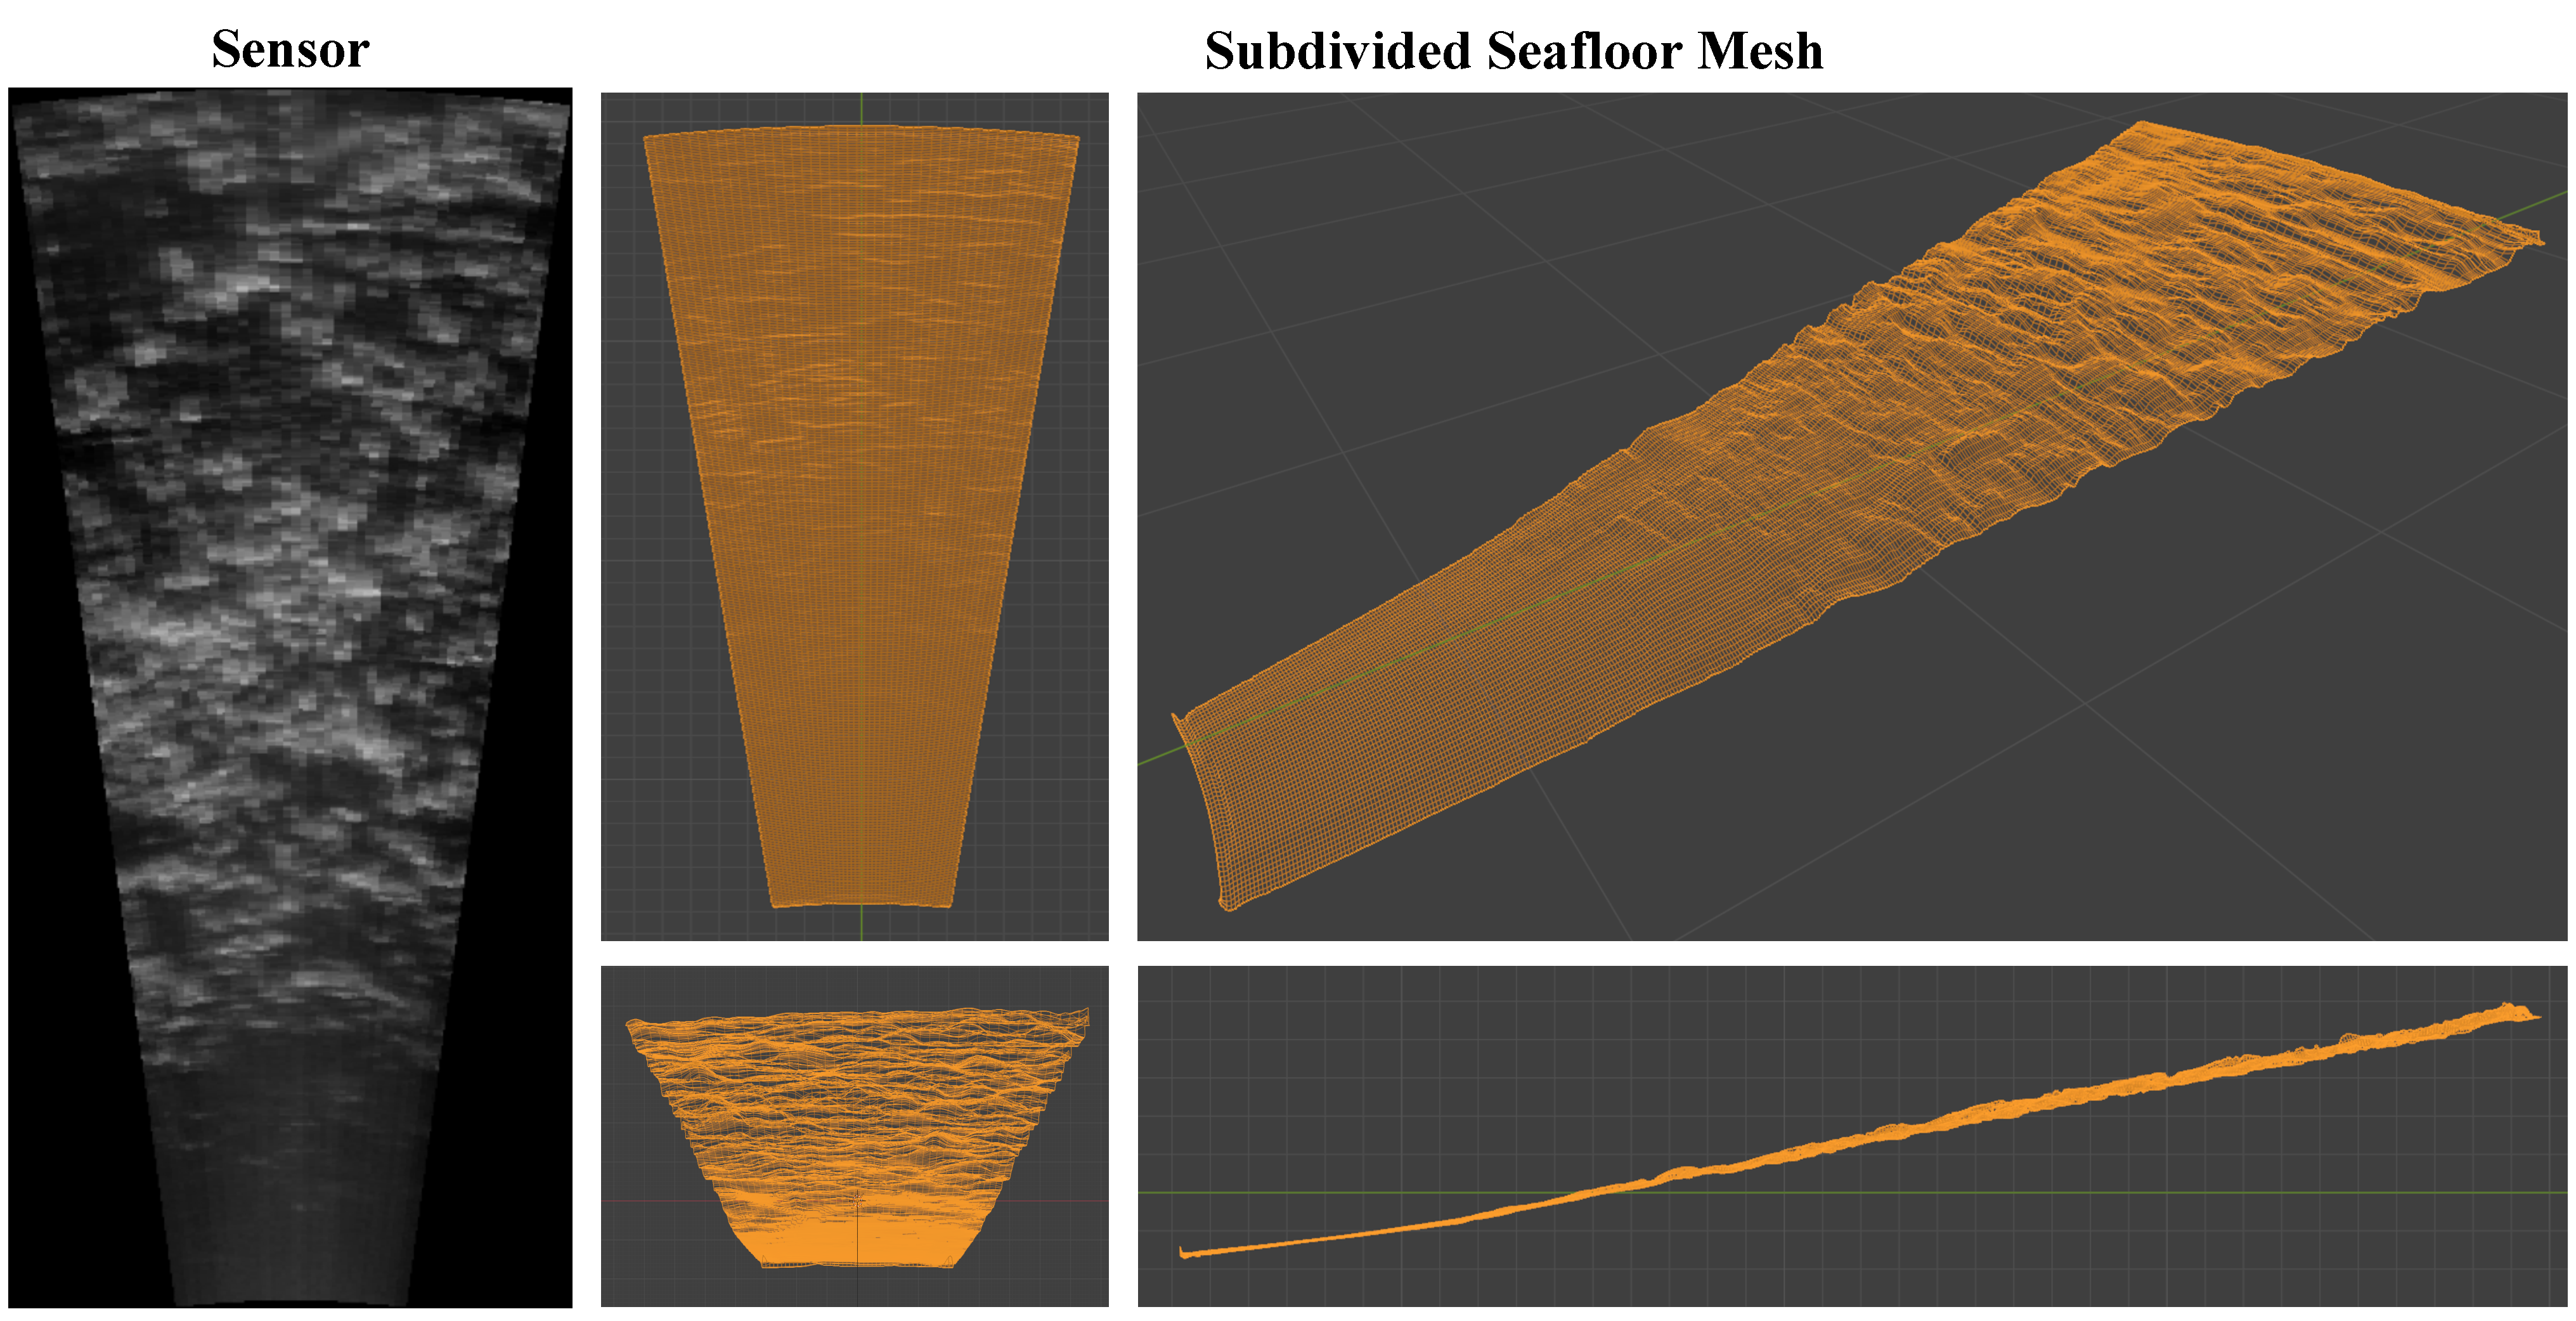
\includegraphics[width=1.0\linewidth]{figs/3d_isometrics_channel.pdf}
    \caption{\centering {\bf Additional views of the recovered seafloor geometry on Kenai Channel} (\textit{cf.} Sec.~\ref{sec:3d_reconstructions}). On the left we show the target again, with additional orthographic views of the recovered height field on the right after one level of Catmull–Clark subdivision in Blender (applied only for visualization).}
    \label{fig:riverB_fig2}
\end{figure*}

\begin{figure*}[t!]
  \centering
  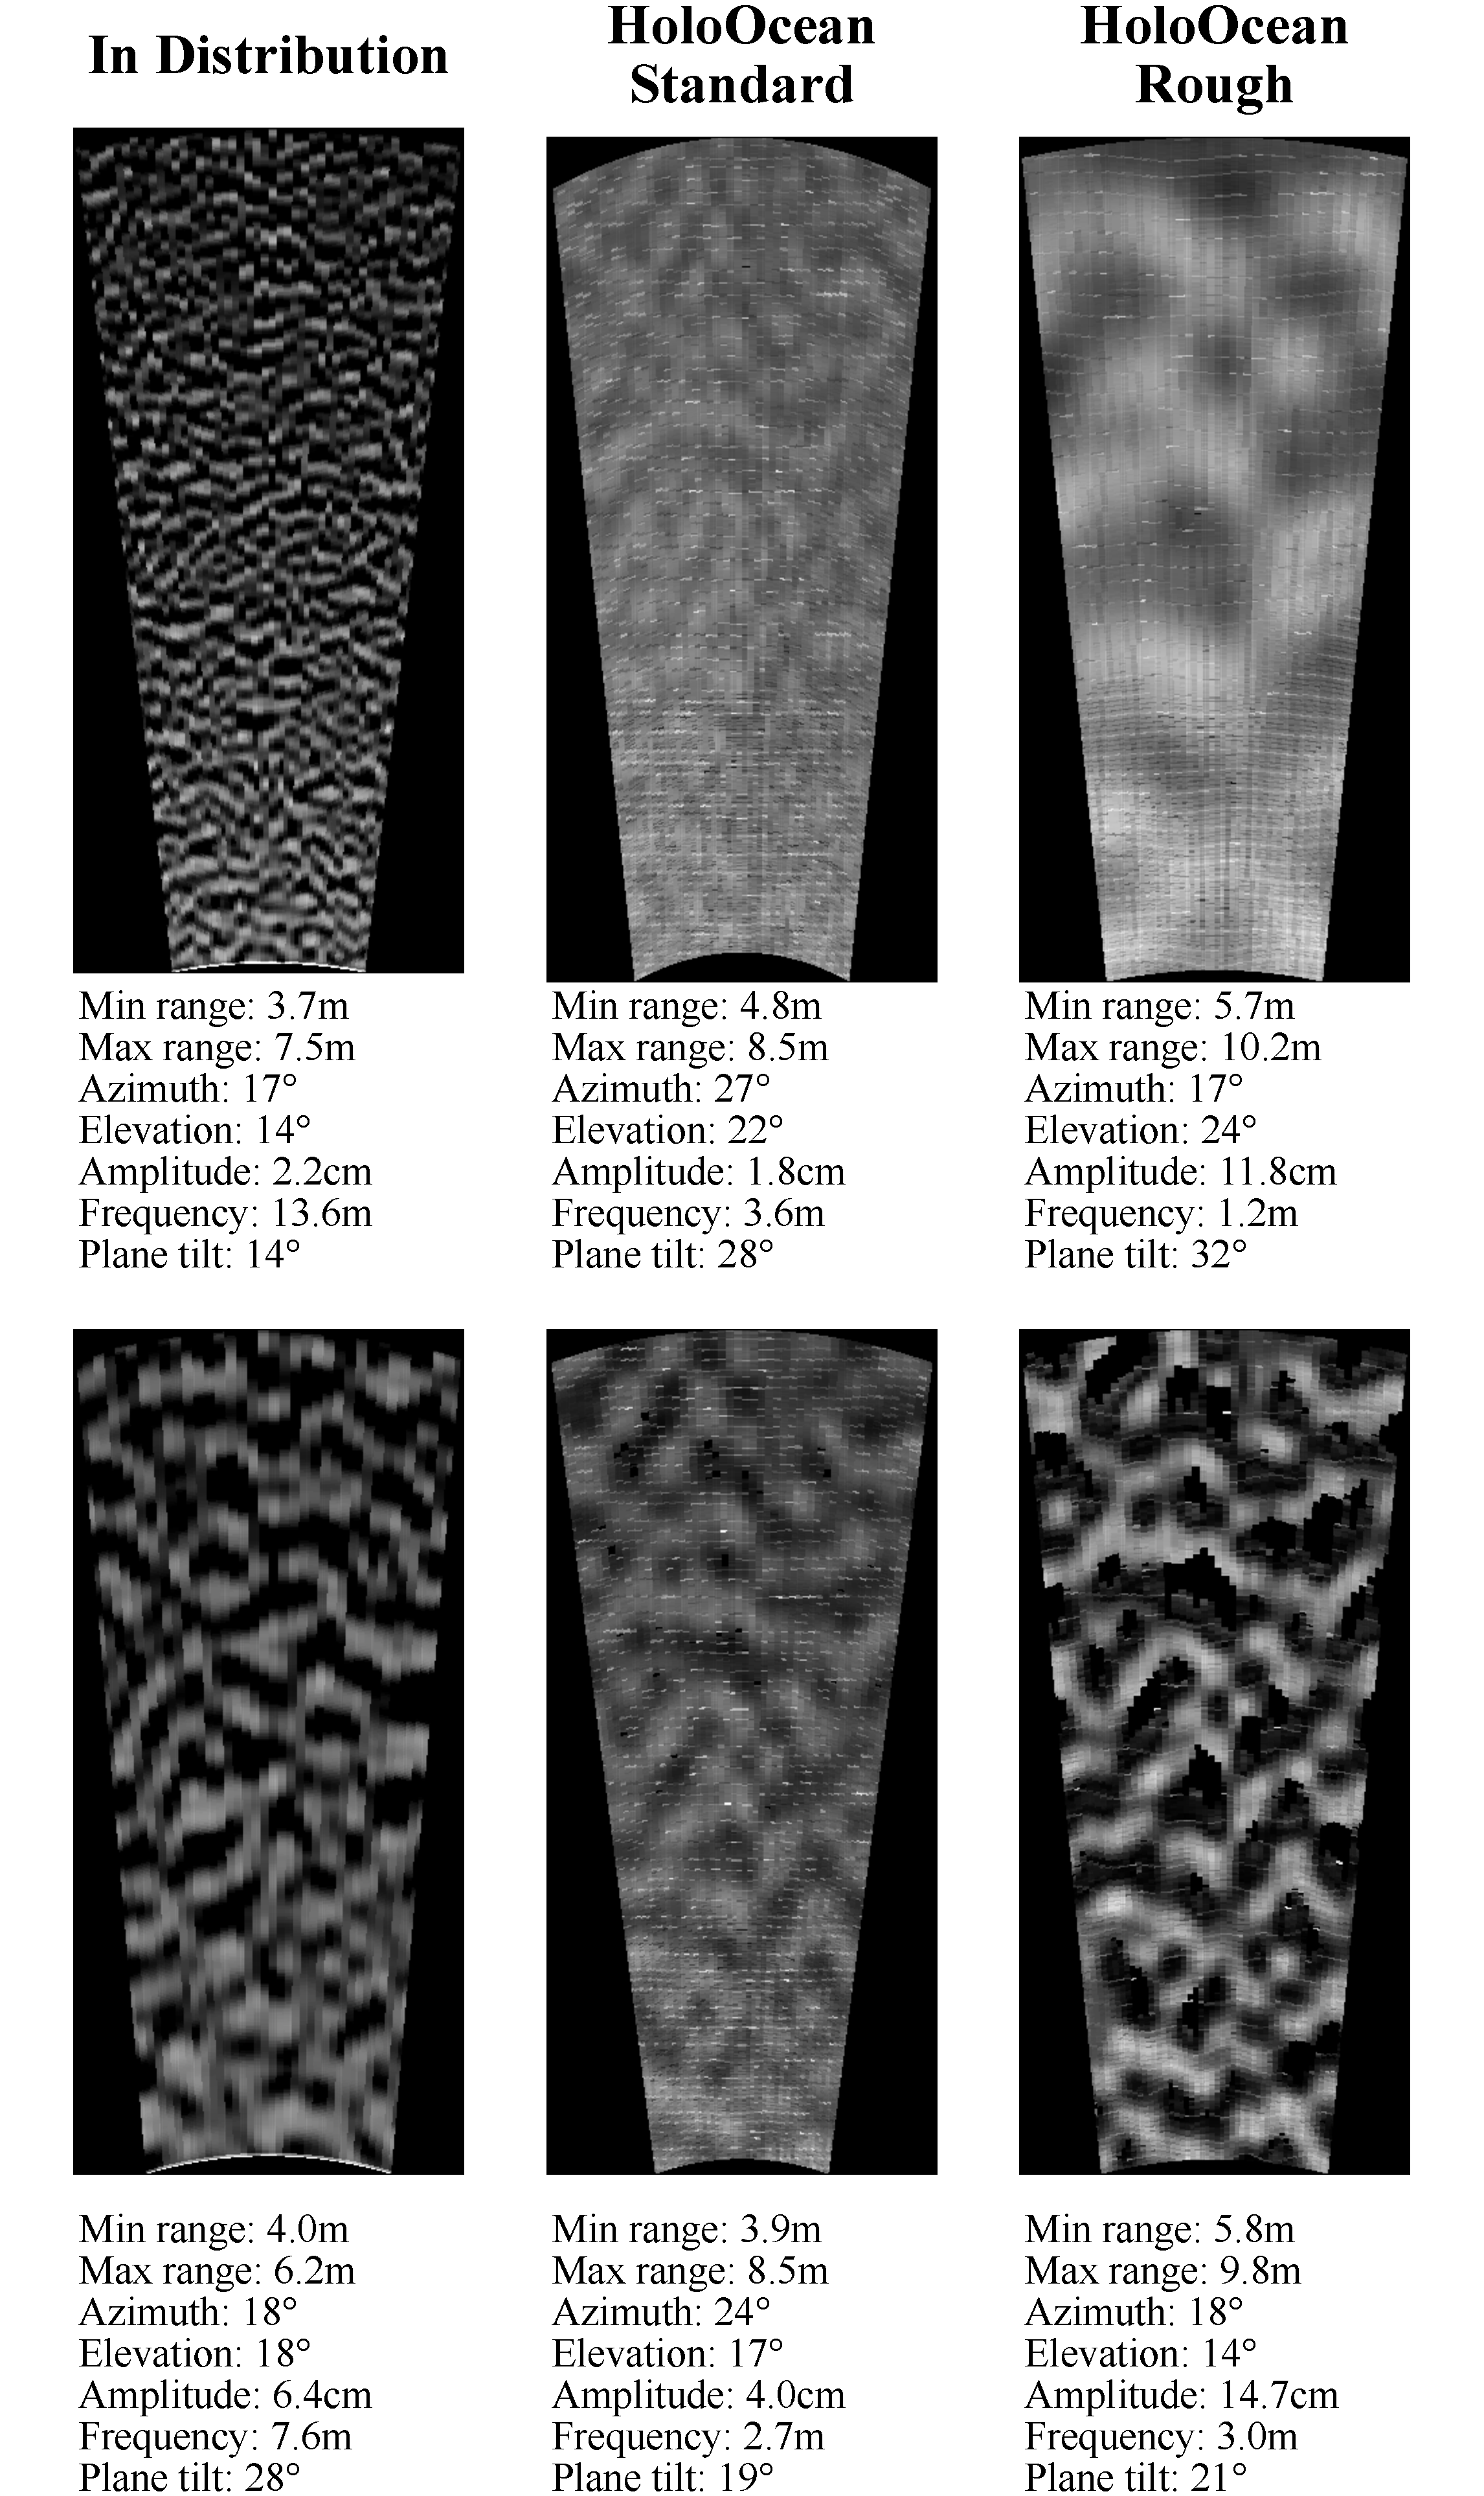
\includegraphics[width=0.75\linewidth]{figs/dataset_samples.pdf}
  \caption{{\bf Example target images from each of our three datasets}. Sampling details can be found in Sec.~\ref{sec:dataset_params}}
  \label{fig:dset_samples}
\end{figure*}
